\subsection{Online Algorithms}

Online \lsa algorithms adopt local checking policies by restricting the distance checking within a sliding or opening window such that there is no need to have the entire trajectory ready before compressing. That is, online algorithms essentially combine {\em batch algorithms} with {\em sliding or opening windows}, \eg\
\opwa \cite{Meratnia:Spatiotemporal} is a combination of top-down algorithm \dpa and opening windows while \kw{SWAB} \cite{Keogh:online} is a combination of bottom-up algorithm \tpa and \textit{sliding windows}.
%
Though these algorithms support the three distance metrics \ped, \sed and \dad, they still have high time and/or space complexities \cite{Liu:BQS}.
%
\textcolor{blue}{Besides, in environments like Wireless Sensor Networks, online algorithms also need to address the problem of balancing the trade-off between the energy cost due to communication and the accuracy of the trajectories’ detection and representation \cite{Ghica:DTracking}, and controlling the ``freshness” (i.e., the latency) of the simplified data by a careful management of the data buffer of an online algorithm \cite{Ghica:DTracking}.}
%
To design more efficient online algorithms, techniques typically need to be designed closely coupled with distance metrics.
Indeed, \bqsa \cite{Liu:BQS} and \squishe \cite{Muckell:Compression} propose to utilize convex hulls and priority queues, respectively, and they speed up trajectory simplification using \ped and \sed, respectively. 
\textcolor{blue}{\dagots~\cite{Cao:Dots} is an online method using \lissed that could be computed in an incremental way, and \olts~\cite{Wu:Graph} has the same idea and methodology as \dagots.}
To our knowledge, no specific techniques have been developed for \dad.
Hence, {\em we choose algorithms \bqsa (\myblue{the performance optimized online algorithm, specific for \ped}), \squishe (\myblue{the famous online algorithm, specific for \sed}), \textcolor{blue}{\dagots (\myblue{the representative of algorithm using \lissed, and is recommended in the recent evaluation work \cite{Zhang:Evaluation}})} and \opwa (\myblue{a well-known online algorithm based on \dpa that is compatible with \dad}) as the representatives of online algorithms using \ped, \sed, \textcolor{blue}{\lissed} and \dad, respectively}.



\subsubsection{Algorithm \opwa \cite{Meratnia:Spatiotemporal}.}
It combines the top-down and opening window strategies, and enforces the constrained global checking in the window. Like \dpa, it supports \ped, \sed and \dad.

Given a trajectory $\dddot{\mathcal{T}}[P_0, \ldots, P_n]$ and an error bound $\epsilon$, algorithm \opwa~\cite{Meratnia:Spatiotemporal} maintains a window $W[P_s, \ldots, P_k]$, where $P_s$ and $P_k$ are the start and end points, respectively. Initially, $P_s$ = $P_0$ and $P_k$ = $P_1$, and the window $W$ is gradually expanded by adding new points one by one. \opwa tries to compress all points in $W[P_s, \ldots, P_k]$ to a single line segment $\mathcal{L}(P_{s}, P_{k})$. If the distances $ped(P_i, {\mathcal{L}})\le \epsilon$ for all points $P_i$ ($i\in[s, k]$), it simply expands $W$ to $[P_s, \ldots, P_k, P_{k+1}]$ $(k+1\le n)$ by adding a new point $P_{k+1}$. Otherwise, it produces a new line segment $\mathcal{L}(P_{s}, P_{k-1})$, and replaces $W$ with a new window $[P_{k-1},\ldots,P_{k+1}]$.  The above process repeats until all points in $\dddot{\mathcal{T}}$ have been considered. The process is similar for \sed and \dad.
%
%\textcolor[rgb]{0.00,0.07,1.00}{According to the different methods of selecting the end points of a line segment, Open Window can further be divided into Normal Penning Window and Before Opening Window~\cite{Meratnia:Spatiotemporal}. When the distance of the point to compressed trajectory exceeds a certain threshold, Normal Opening Window algorithm select that point as the end point, while Before Opening Window select the last point within the window as the end point of the current trajectory.}
%
The time complexity of algorithm \opwa remains in $O(n^2)$ tim, the same as the \dpa algorithm.


\subsubsection{Algorithm BQS Using \ped \cite{Liu:BQS}}
It is essentially an efficiency optimized \opwa algorithm \cite{Meratnia:Spatiotemporal}, and reduces the running time by introducing convex hulls to pick out a certain number of points, which makes it dedicated for \ped.

For a buffer $W$ with sub-trajectory $[P_s, \ldots, P_k]$, it splits the space into four quadrants. A buffer here is similar to a window in \opwa \cite{Meratnia:Spatiotemporal}. For each quadrant, a rectangular bounding box is firstly created using the least and highest $x$ and $y$ values among points $\{P_s,\ldots,P_k\}$, respectively. Then another two bounding lines connecting points $P_s$ and $P_{h}$ and points $P_s$ and $P_{l}$ are created such that lines $\vv{P_sP_{h}}$ and $\vv{P_sP_{l}}$ have the largest and smallest angles with the $x$-axis, respectively.
Here $P_{h},P_{l} \in\{P_s,\ldots,P_k\}$. The bounding box and the two lines together form a convex hull.
Each time a new point $P_k$ is added to buffer $W$, \bqsa first picks out at most eight significant points from the convex hull in a quadrant. It calculates the distances of the significant points to line $\vv{P_sP_k}$, among which the largest distance $d_{u}$ and the smallest distance $d_l$ are an upper bound and  a lower bound of the distances of all points in $[P_s, \ldots, P_k]$ to line $\vv{P_sP_k}$.
(1) If $d_l\ge \epsilon$, it produces a new line segment $\mathcal{L}(P_{s}, P_{k-1})$, and produces a new window $[P_{k-1},\ldots,P_{k}]$ to replace $W$.
(2) If $d_u < \epsilon$, it simply expands buffer $W$ to $[P_s, \ldots, P_k, P_{k+1}]$ $(k+1\le n)$ by adding a new point $P_{k+1}$.
(3) Otherwise, it computes all distances $d(P_i, {\mathcal{L}(P_s,P_k)})$ ($i\in[s, k]$) as algorithm \dpa does.
%
The time complexity of \bqsa remains $O(n^2)$. However, its simplified version \fbqsa has a linear time complexity by essentially avoiding case (3) to speed up the process.


\begin{figure}[tb!]
	%\vspace{-1ex}
	\centering
	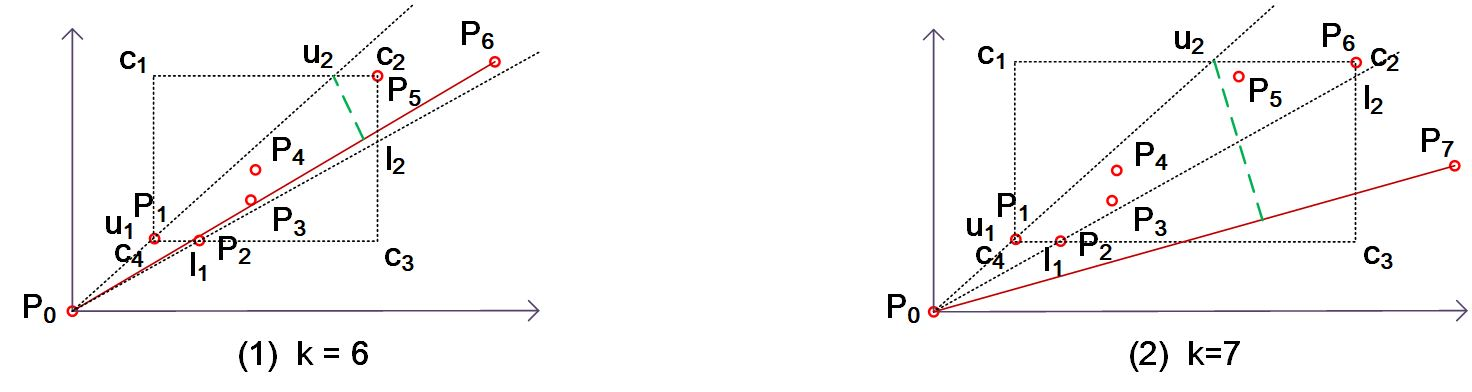
\includegraphics[scale = 0.66]{Figures/Fig-BQS.jpg}
	\vspace{-1ex}
	\caption{{\small Examples for algorithm \bqsa.}}
	\label{fig:bqs}
	\vspace{-2ex}
\end{figure}


\begin{example}
	\label{exm-alg-bqs}
	Figure~\ref{fig:bqs} is an example of \bqsa. The bounding box $c_1c_2c_3c_4$ and the two lines $\vv{P_sP_{h}} = \vv{P_0P_1}$ and $\vv{P_sP_{l}} = \vv{P_0P_2}$ form a convex hull $u_1u_2c_2l_2l_1c_4$. \bqsa computes the distances of $u_1,u_2,c_2,l_2,l_1$ and $c_4$ to line $\vv{P_0P_6}$ when $k=6$ or to line $\vv{P_0P_7}$ when $k=7$.
	%
	When $k=6$, all these distances to $\vv{P_0P_6}$  are less than $\epsilon$, hence \bqsa goes on to the next point (case 2); When $k=7$,
	the max and min distances to $\vv{P_0P_7}$ are larger and less than $\epsilon$, respectively, and \bqsa needs to compress sub-trajectory $[P_0, \ldots, P_7]$ along the same line as \dpa (case 3).
\end{example}




\subsubsection{Algorithm SQUISH-E Using \sed~\cite{Muckell:Compression}}
It is an online bottom-up algorithm that is {dedicated for \sed}, and has two forms: \squishe($\lambda$) ensuring the compression ratio $\lambda$, and \squishe($\epsilon$) ensuring the \sed error bound $\epsilon$. Here we adopt \squishe($\epsilon$), as we focus on error bounded trajectory simplification.

\eat{%%%%%%%%%%%%%%%%
taking as input a trajectory \trajec{T} and two additional parameters $\lambda$ and $\epsilon$.
It first compresses trajectory \trajec{T} while striving to minimize \sed error and achieving the compression ratio of $\lambda$. Then, it further compresses \trajec{T} as long as this compression will not increase the max \sed error beyond $\epsilon$.

Meanwhile, \squishe($\lambda$) is the case where $\epsilon$ is set to $0$ and therefore it minimizes \sed error ensuring the compression ratio of $\lambda$, and
\squishe($\epsilon$) denotes another case, \ie the \emph{min-$\#$ problem}, where $\lambda$ is set to $1$ and therefore it maximizes compression ratio while keeping \sed error under $\epsilon$.
In this paper, we only discuss \squishe($\epsilon$).
}%%%%%%%%%%%%%%%%%%%%

Algorithm \squishe optimizes algorithm \tpa with a doubly linked list $Q$. Each node in the list is a tuple $P(pre, suc, mnprio, prio )$, where $P$ is a trajectory data point, $pre$ and $suc$ are the predecessive  and successive points of $P$, respectively,  $prio$ is the priority of $P$ defined as an upper bound of the \sed error that the removal of $P$ introduces, and $mnprio$ is the max priority of its predecessive and successive points removed from the list.
%
Initially, trajectory points are loaded to $Q$ one by one.
At the same time, $mnprio$ of each point is set to $zero$ as no node has been removed from the list.
Moreover, the priorities of points $P_0$ and $P_{|Q|-1}$ are set to $\infty$, and the priority of point $P_i$ ($0<i<|Q|-1$) is set to $sed(P_i, \vv{pre(P_{i})suc(P_{i})})$.
%
Then, \squishe finds and removes a point $P_j$ from $Q$ that has the lowest priority $prio(P_j)<\epsilon$, and the properties $mnprio$ of predecessor $pre(P_j)$ and successor $suc(P_j)$ are updated to $\max(mnprio(pre(P_j)), prio(P_j))$ and $\max(mnprio(suc(P_j)), prio(P_j))$, respectively.
Next, the properties $prio$ of $pre(P_j)$ and $suc(P_j)$ are further updated to $mnprio(pre(P_j))$ + $sed(pre(P_j), \vv{pre(pre(P_{j}))suc(P_{j})})$ and $mnprio(suc(P_j))$ + $sed(suc(P_j),\vv{pre(P_{j})suc(suc(P_{j}))})$, respectively.
%
After that, a new point is read to the list and the information of its predecessor in the list is updated.
%
The above process repeated until that no points have a priority smaller than $\epsilon$.
%
\squishe finds and removes a point from $Q$ that has the lowest priority in $O(\log |Q|)$ time, where $|Q|$ denotes the number of points stored in $Q$.
Thus, \squishe runs in $O(n\log |Q|)$ time and $O(|Q|)$ space.



\begin{figure*}[tb!]
	\centering
	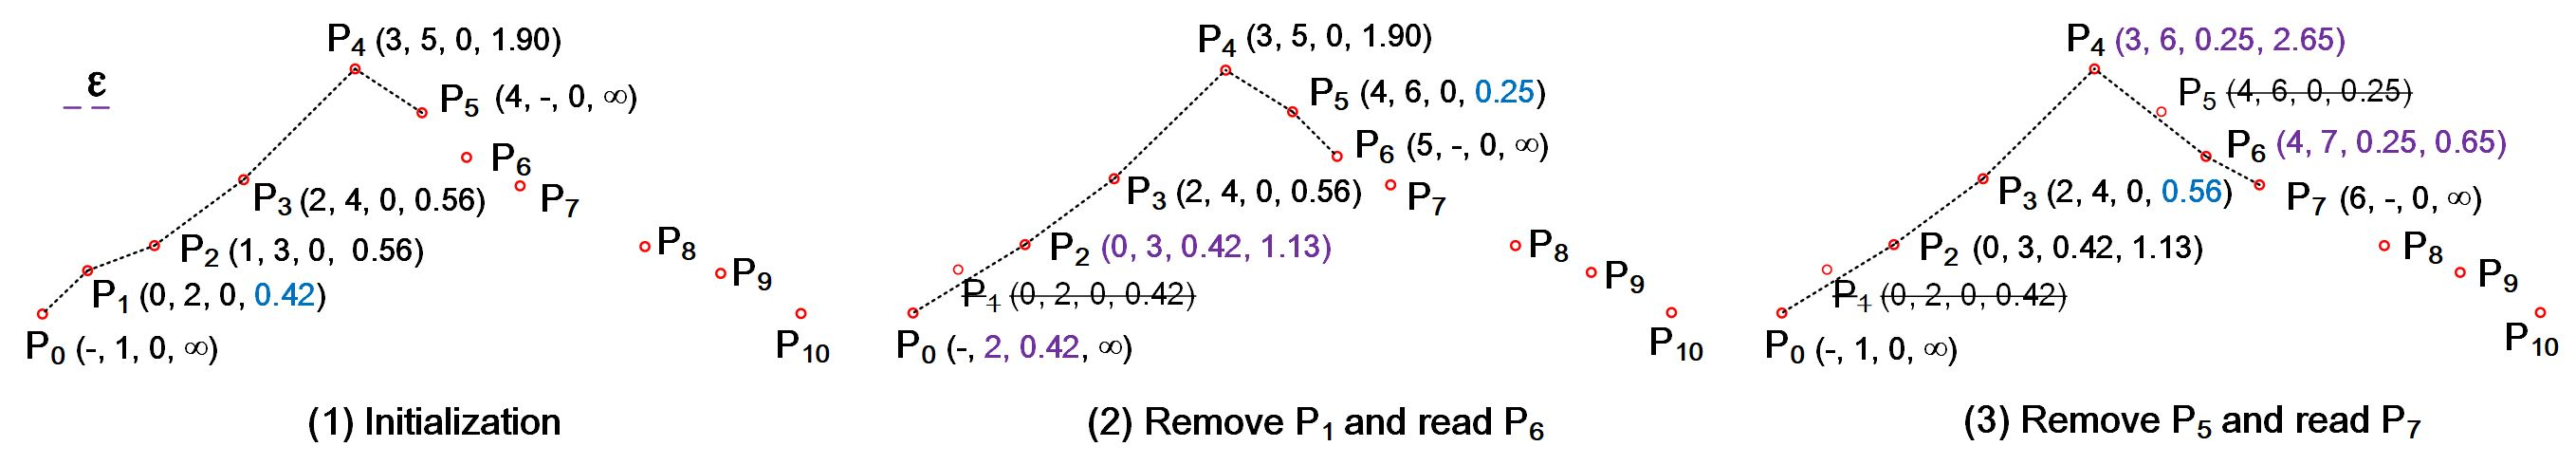
\includegraphics[scale=0.48]{Figures/Fig-Squishe.jpg}
	\vspace{-2ex}
	\caption{\small The trajectory $\dddot{\mathcal{T}}[P_0, \ldots, P_{10}]$ is compressed by the \squishe algorithm using \sed to five line segments. The size of Q is 6, and the data structure after point $P$ is a tuple $(pre, suc, mmprio, prio)$. }
	\vspace{-1ex}
	\label{fig:squishe}
\end{figure*}



\begin{example}
	\label{exm-alg-squishe}
	Figure~\ref{fig:squishe} is an example of \squishe.
	%
	(1) Initially, $|Q| = 6$ points are read to the list. The tuple $(pre, suc, mmprio, prio)$ for each point is initialized. For example, the tuple of $P_1$ is set to $(0, 2, 0, 0.42\epsilon)$, where $0.42\epsilon$ is the \sed from $P_1$ to $\vv{P_0P_2}$.
	%
	(2) The priority of $P_1$ has the minimal value, thus, it is removed from the list.
	The $mnprio$ properties of $P_0$ and $P_2$ are updated to $max\{mnprio(pre(P_1)), prio(P_1)\}$ = $max\{mnprio(P_0), prio(P_1)\}$ = $max\{0, 0.42\epsilon\}$ = $0.42\epsilon$, and $max\{mnprio(P_2), ~prio(P_1)\}$ = $0.42\epsilon$, respectively.
	Furthermore, the $prio$ property of $P_2$ is updated to $mnprio(suc(P_j)) + sed(suc(P_j),\vv{pre(P_{j})suc(suc(P_{j}))})$ = $mnprio(P_2) + sed(P_2,\vv{P_0P_3})$ = $0.42\epsilon + 0.71\epsilon$ = $1.13\epsilon$, and the $prio$ property of $P_0$ is still $\infty$.
	Then, $P_6$ is read, and the information of $P_5$ is updated.
	%
	(3) $P_5$ is removed and $P_7$ is read to the list.
	%
	(4) {Finally, the algorithm outputs 5 line segments $\vv{P_0P_2},\vv{P_2P_4},\vv{P_4P_7},\vv{P_7P_9}$ and $\vv{P_9P_{10}}$}.
\end{example}

\subsubsection{\textcolor{blue}{Algorithm DOTS Using \lissed~\cite{Cao:Dots}}}
\textcolor{blue}{It is a directed acyclic graph based online trajectory simplification method that supports \lissed. Other than the optimal and near optimal algorithms \cite{Chen:Fast,Daescu:metric} that first construct the reachability graph then find a shortest path from it, \dagots~determines part of the shortest path when constructing preceding part of the whole graph \cite{Cao:Dots}.}
%, \ie it runs in a recursive manner.
%before the whole graph is completely constructed, 

\textcolor{blue}{It first shows that, in this problem, the reachability graph of an input trajectory finally retrogrades to a tree structure. It also observes that the local approximation error $lissed(P_s,P_{s+k})$ is growing with respect to $k$, thus, it is ``reasonable" to assume that $k$ should not be too large. 
By this assumption, each layer of the tree could be added without feeding the entire trajectory, and the shortest path could also be determined recursively, \ie layer by layer.}
%
\textcolor{blue}{For each node (point) in each layer, \dagots~marks those having descendants as \emph{alive} and others as \emph{dead}.
Initially, the first layer $Q_0$ is $\{P_0\}$, and it is \emph{alive}. }
%
\textcolor{blue}{Then, let $c>0$ and $Q_c$ is the current layer under construction, 
\dagots~in turn adds point $P_{s+k}$, having a \lissed distance to any point of $Q_{c-1}$ less than error bound, to $Q_c$, until no point can be added to $Q_c$ (remember $k$ should not be too large). After that, it updates the status of each layer that has \emph{alive} points: the parent of an \emph{alive} point may be adjusted to minimize the total integral square \sed of the path, points without descendants will be marked as \emph{dead}, and those 1-alive-element layers will be decoded and their \emph{alive} points will be output to the simplified trajectory. }
%
\textcolor{blue}{The time complexity of \dagots~is $O(n^2/K)$, where K is the number of output points, and the space complexity of \dagots~is $O(|Q|^2)$, where $|Q|$ is the size of a layer.}

\begin{figure*}[tb!]
	\centering
	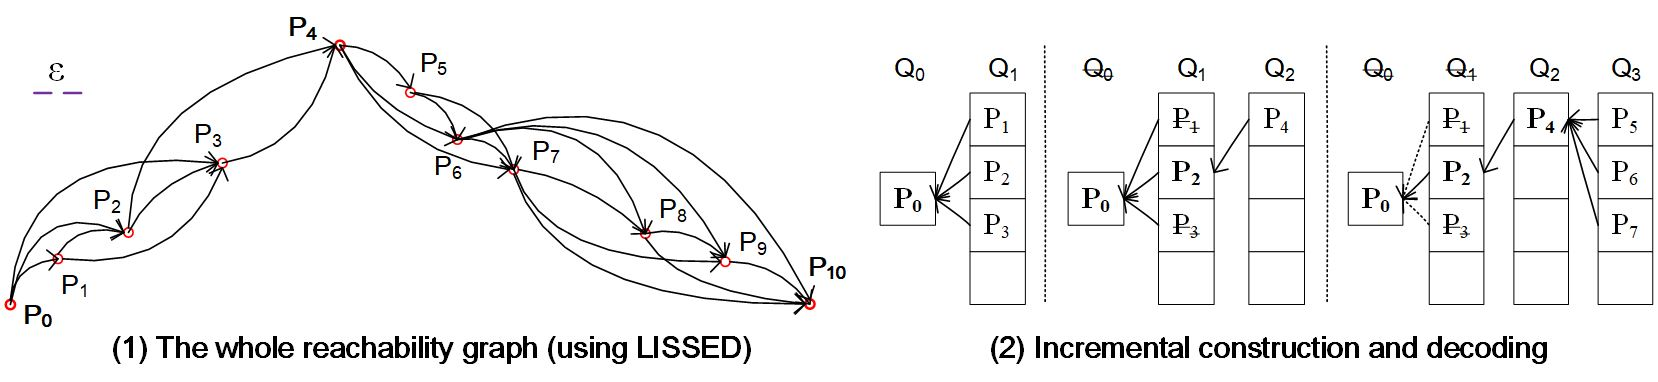
\includegraphics[scale=0.79]{Figures/Fig-DOTS.jpg}
	\vspace{-2ex}
	\caption{\small \textcolor{blue}{Example of algorithm \dagots~using \lissed with error bound of $\epsilon^2$, where (1) left is the supposed reachability graph of trajectory $\dddot{\mathcal{T}}[P_0, \ldots, P_{10}]$, and (2) right is the incremental construction of reachability graph and online decoding of the shortest path. Finally, the trajectory is compressed to four line segments.} }
	\vspace{-1ex}
	\label{fig:dots}
\end{figure*}



\begin{example}
	\label{exm-alg-dots}
	\textcolor{blue}{Figure~\ref{fig:dots} is an example of \dagots. The reachability graph is constructed layer by layer incrementally, and part of the shortest path is determined before the whole graph is completely constructed. }
	%
	(a) \textcolor{blue}{Initially, $P_0$ is added to the first layer $Q_0$, and it's the only element in the layer.}
	%
	(b) \textcolor{blue}{Then, points $P_1$, $P_2$ and $P_3$ are in turn added to the second layer $Q_1$. Because $P_0$ does not have any new child point, \dagots~updates the status of $Q_1$ and outputs $P_2$ as it is the only \emph{alive} point in $Q_1$.}
	%
	(c) \textcolor{blue}{The process repeat. Point $P_4$ is added to layer $Q_2$, points $P_5$, $P_6$ and $P_7$ are added to layer $Q_3$, and so on.  }
	%
	(d) \textcolor{blue}{Finally, it outputs 4 line segments $\vv{P_0P_2},\vv{P_2P_4},\vv{P_4P_7}$ and $\vv{P_7P_{10}}$.}
\end{example}

%%%%%%%%%%%%%%%%%%%%%%%%%%%%%%%%%%%%%%%%%%%%%%%%%%%%%%%%%%%%%%%%%%%%% END %%%%%%%%%%%%%%%%%%%%%%%%%%%%%%%%%%%%%%%%%%%%%%%%%%%%%%%%%%%%%%%%%%%%%%%%%%



\eat{%%%%%%%%%%%%%%%%%%%%%%%%%%%%%%%%%%%%%%%%%%%%%%%%%%%%%%%

\subsubsection{Sliding Window and Bottom-up}

The \swab algorithm~\cite{Keogh:online} is essentially the combination of the Sliding Window mechanism and the Bottom-up algorithm.
It keeps a window, $w[P_s, \ldots, P_{s+k-1}]$, of a fixed size of $k$.
The window size $k$ should be carefully chosen so that there are enough data points in the window to create about 5 or 6 line segments \cite{Keogh:online}.
Initially, $P_s=P_0$.
Next, the Bottom-Up algorithm, \eg \pavlidis algorithm, is applied to the points in the window, which merges the points into segments with the left-most segment being $\vv{P_sP_{s+i}}$, $i<k$.
Then $\vv{P_sP_{s+i}}$ is output, the window slides to right taking $P_{s+i+1}$ as the new start point of the window, and the Bottom-Up algorithm is applied again.
This process repeated until all points have been merged to segments.

The time complexity of \swab is a small constant factor worse than that of the standard Bottom-Up algorithm~\cite{Keogh:online}.
Also, it supports \sed. % as the standard Bottom-Up algorithm does.

\textcolor[rgb]{1.00,0.00,0.00}{Todo...dis-continuous line segments.}

} %%%%%%%%%%%%%%%%%%%%%%%%%%%%%%%%%%%%%% End of eat

